\documentclass{article}
\usepackage{graphicx} % Required for inserting images
\usepackage[rightcaption]{sidecap}
\usepackage[style=alphabetic]{biblatex}

\graphicspath{ {./images/} }
\addbibresource{sample.bib}

\title{Assignment 4 Report}
\author{Ole Rößler (7211)}
\date{December 2024}

\begin{document}

\maketitle
\tableofcontents

\newpage
\section{Design Exercise: Flight Booking System}

\subsection{Requirements}
This section talks about the functional and non-functional requirements of the flight booking system wanted by the ACME Organization. 
The main points given were about the given points considering (this will be a short overview about the task).

Short Description what the differences between function and non-function requirements are and I chose them (from the given context and my personal thought).

\subsubsection{Functional Requirements}
\begin{enumerate}

\item \textbf{Fetching Data:}
Periodically receive flight data updates from partner airlines (every hour).
\item \textbf{View Flights:}
The customer is able to see specific flight details. 
Therefore the customer enters a specific flight number/ flight ID and gets updates about the specified flight.
\item \textbf{Booking:}
The customer is able to book a flight on a desired flight as well as make a seat reservation on the airplane (Most airlines offer different price-tiers for seats). 
\end{enumerate}

\subsubsection{Non-Functional Requirements}
\begin{enumerate}
\item \textbf{Price Consistency:}
The system has to maintain consistency in pricing, therefore short term increases in flight-prices have to be avoided .
\item \textbf{Performance:}
Low latency for user interactions (response within seconds).
\item \textbf{Scalability:}
The system has to handle hundreds of thousands of concurrent users as well as hundreds of flights send in their data on the hour.
\item \textbf{Fault tolerance:}
The system has to be reliable.
\end{enumerate}

\subsection{System Architecture}
\begin{figure}
    \centering
    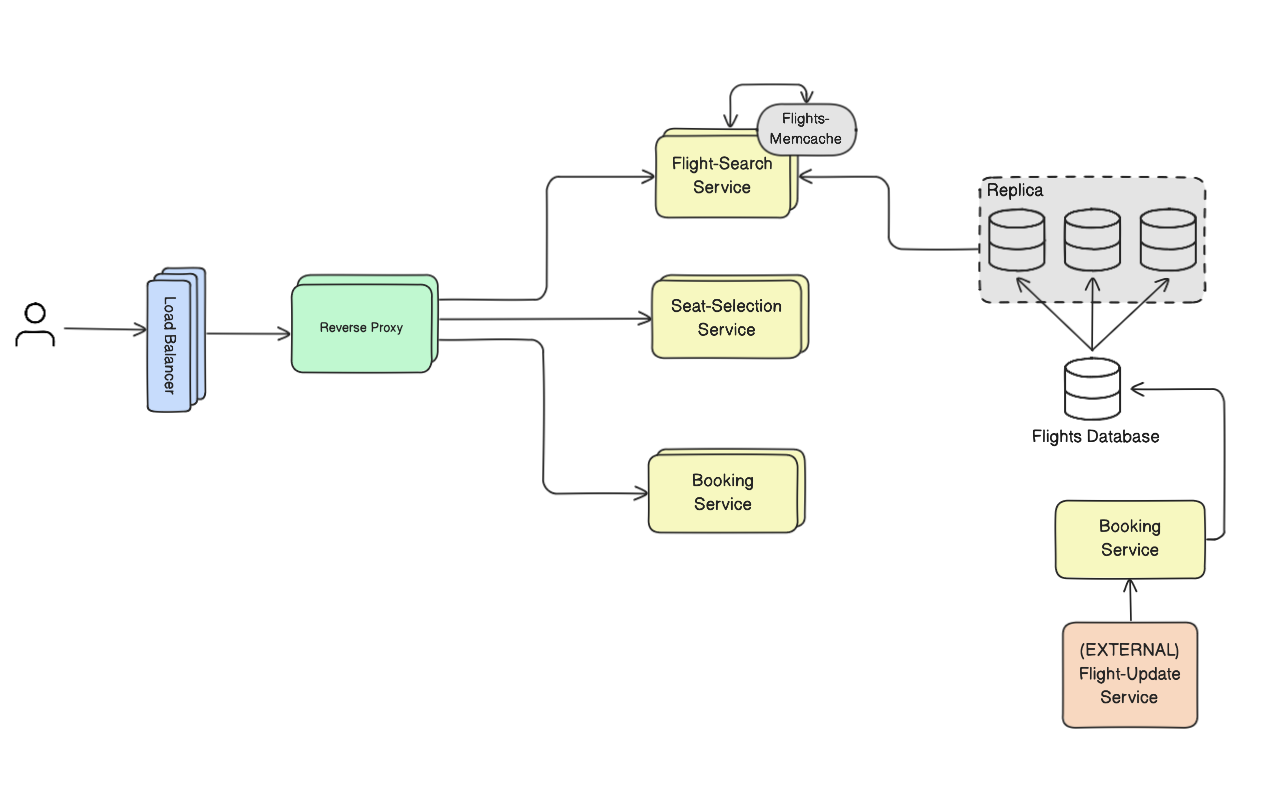
\includegraphics[width=\linewidth]{1st_system_design_sketch.png}
    \caption{Redesigned flight booking system (FBS)}
    \label{fig:enter-label}
\end{figure}
\newpage 

\subsection{Discussion}
The functional requirements are mainly implemented as micro-services.
The Flight-Search service queries the database according to the users flight-data. The booking service is used to book a flight that 

The Seat-Select service is called if a customer wants to make a seat reservation on a selected plane. 
The proxy handles...security before forwarding to service, also record performance metrics as entry-point???

In order to address the non-functional requirements and insure scalability and performance different measures were taken. 
The Load-Balancer distributes the incoming traffic equally to the proxy-servers so that the performance of the system isn't impacted by a single overloaded server (that would take way to long to respond to the user-requests). This also enables another point of scalability such that we can increase the number of proxy servers if the overall workload is to high.
My analysis of the given flight-booking-system was, that it has a high write-to-read ratio (meaning the number of writes is way higher than the number of reads). Therefore we have database dublicates that all follow a single leader. With the additional caching it is insured, that the database-reads don't bottleneck the application. In the future additional replica can be added to support the database layer. We could also add additional partitioning (by origin-destination). 

To scale the micro-services it is always possible to horizontally scale the micro-services by adding more instances. If the request arrives at the service it will be load-balanced internally and send to one of its instances.


\section{Freestyle Exercise}
\subsection{My DS-Concept}
I chose to implement a distributed version of our assignment server. 
The core improvement is, that the workload is distributed amongst various stateless servers that can access a database to update a representative "assignment-01"-score. To scale the number of servers horizontally, I implemented a loadbalancer that uses round-robin scheduling to distributes the work amongst the registered servers. The idea is that the clients can only communicate with the servers via the loadbalancer, that forwards the workload, therefore increasing the maximum number of requests that can be processed in parallel. 
To represent a distributed system on a local machine, I wrote a docker-com 

I chose to model two different networks (net-1 and net-2) representing different data-centers. 

that is able to detect nodes that fail and automatically replaces them.
->read/write to database 
->basic flight protocol, i can receive flight information and write to the database using ???

\subsection{Evaluation}
Round-robin loadbalancing is enough for our usecase, but can could be more optimal(utilization based).

Pros:
read/write balance is good, way less writes than reads, therefore single leader is enough for handliung the writes.

Reads is way higher, because (problem, currently i write even on fail). 
HEARTBEAT:
- If a server is shut down or physically seperated from the load-balancer for any reason, the implemented udp-heartbeat can't be received by the load-balancer. Therefore the server is removed from the list of servers, participating in the round-robin.
servers



->Discussion Points
-Exposing API?

big minus SECURITY:
-> API has no verificaction e.g. bearer token,e.g.
-> Single point of failure in loadbalancer and 

Improvements:
-> Distributed database 
-> Modularity/Encapsiation: Have api layer between db and java servers

\printbibliography[heading=bibintoc]
\end{document}
